\documentclass[A4paper,12pt]{article}

% --- Math & fonts ---
\usepackage[centertags]{amsmath}
\usepackage{amsfonts}
\usepackage{amssymb}
\usepackage{amsthm}
\usepackage{latexsym}
\usepackage{mathptmx}

% --- Graphics & figures ---
\usepackage{graphicx}
\usepackage{epsfig}
\usepackage{epstopdf}
\usepackage{float}
\usepackage{placeins}
\usepackage{caption}
\usepackage{adjustbox}
\usepackage{rotating}
\usepackage{lscape}

% --- Colors, frames & boxes ---
\usepackage[table,xcdraw]{xcolor}
\usepackage{framed}
\usepackage{fancybox}
\usepackage{color}

% --- Tables ---
\usepackage{booktabs}
\usepackage{threeparttable}

% --- Formatting ---
\usepackage{newlfont}
\usepackage{setspace}
\usepackage{kantlipsum}
\usepackage{fancyhdr}
\usepackage[normalem]{ulem}
\useunder{\uline}{\ul}{}

% --- Page layout ---
\usepackage[hmargin=1.4in,vmargin=1.4in]{geometry}

% --- References with natbib ---
\usepackage[numbers,sort&compress]{natbib}
\bibliographystyle{unsrt}

\setlength{\parindent}{0pt}
\setlength{\parskip}{1em} % adds vertical space between paragraphs

\newgeometry{left=1in,right=1.0in,top=1.0in,bottom=1in}
\setlength\extrarowheight{6.5pt}

\pagestyle{fancy}
\fancyhf{}
\renewcommand{\headrulewidth}{0pt}
\renewcommand*\FrameCommand{\hskip0.6cm\fcolorbox{black}{white}}%
\newlength{\framedline}
\setlength{\framedline}{0.966\textwidth}
\let\oldrule\rule
\renewcommand{\rule}[2]{
	\hspace*{-6.3pt}\oldrule{\framedline}{0.4pt}\newline}
\linespread{1.213}

\begin{document}

\begin{center}

\textsc{\huge COMSATS University Islamabad \\[0.6cm] Attock Campus}\\[0.6cm]


\includegraphics[height=3.5cm]{comsats.jpg}

\vspace{0.8cm}

{\LARGE \textbf{Project Proposal}}\\[0.8cm]

for\\[0.8cm]

{\LARGE \textbf{Jawhar: AI-Powered Classical Arabic \& Quranic Learning Platform}}\\[0.8cm]

by\\[0.4cm]

\textbf{Meher Ali} \\[0.2cm]
\textbf{Hammad Ali} \\[0.8cm]

CIIT/FA23-BCS-059/ATK \\[0.2cm]
CIIT/FA23-BCS-007/ATK \\[1.2cm]

\textbf{Supervisor}\\[0.4cm]
\textbf{Mr. Babar Shahzad}\\[3cm]

\textbf{Bachelor of Science in Artificial Intelligence / Computer Science (2022--2026)}

\end{center}

\newpage
\begin{center}

\LARGE{\textbf{Jawhar: AI-Powered Classical Arabic \& Quranic Learning Platform}}\\
\vspace{0.5in}

\normalsize{By}\\
\vspace{0.5in}
\large{\textit{Meher Ali}\\
{\textit{CIIT/FA23-BCS-059/ATK}}}\\
\large{\textit{Hammad Ali}\\
{\textit{CIIT/FA23-BCS-007/ATK}}}\\
\vspace{0.5in}

\normalsize{As the supervisor, I have reviewed the proposed project and found it to be feasible, relevant, and aligned with academic and industry standards. I recommend this project for evaluation by the committee to assess its viability and approval for further development.}\\
\end{center}

\vspace{0.1in}

Supervisor Signature:\line(1,0){280}
\begin{center}
\normalsize{Mr. Babar Shahzad\\
Department of Computer Science, (CUI) Attock Campus}
\end{center}
\vspace{0.1in}
\newpage

\pagenumbering{gobble}
\cfoot{\thepage}
\pagenumbering{arabic}
\medskip

\section*{\fontsize{16}{12}\selectfont Project Summary}
This project presents \textbf{Jawhar}, an AI-powered Classical Arabic and Quranic learning platform engineered to bridge a fundamental pedagogical and technological divide. Over 1.8 billion Muslims globally engage with the Quran, yet fewer than 20\% possess the linguistic capability to understand its original Classical Arabic syntax and morphology. Existing solutions either oversimplify instruction into basic vocabulary flashcards (e.g., Quranic, Kalaam) without grammar, or exist as complex, desktop-only computational corpora (e.g., corpus.quran.com) tailored strictly for linguistic researchers. 

Jawhar resolves this dilemma by unifying natural language processing (NLP) architectures with cognitive learning theory into an intuitive, multiplatform application. The system integrates three foundational AI modules: (i) an automated \textbf{Sarf Engine} powered by CAMeL Tools for 3-letter root extraction, morphological pattern (Awzan) identification, and verb conjugation; (ii) an interactive \textbf{Nahw Parser} utilizing Farasa and traditional I'rab frameworks to render color-coded syntactic dependencies; and (iii) an intelligent, pedagogically guarded \textbf{AI Tutor} powered by Gemini Flash that delivers context-aware grammatical explanations with verified Quranic proofs. To guarantee long-term retention, vocabulary acquisition is driven by a spaced repetition system (SRS) implementing modern memory retention modeling. Developed with a high-performance Python FastAPI backend and a shared Kotlin Multiplatform client (targeting Android, iOS, Desktop, and Web), Jawhar democratizes scholarly Quranic linguistics for self-paced global learners.

\newpage
\pagestyle{fancy}

\section{Introduction}
Understanding the Holy Quran in its original liturgical language requires mastery of Classical Arabic (CA). Classical Arabic differs fundamentally from Modern Standard Arabic (MSA) and vernacular dialects, exhibiting an intricate root-and-pattern morphological system (\textit{Sarf}) and a highly inflected, case-sensitive syntactic dependency structure (\textit{Nahw}). Because Arabic is a fusional language where prefixes, stems, and suffixes merge into complex tokens (e.g., \textit{fasayakf{\=i}kahum}), a single vowel or diacritic error (\textit{harakah}) can completely alter the semantic or theological meaning.

Traditional methods of learning Classical Arabic demand years of intensive, synchronous study under expert linguists. Modern digital tools have attempted to address this demand, but have fractured the learning experience. General-purpose language apps such as Duolingo and Babbel focus on modern conversational dialects and neglect classical grammar entirely. Meanwhile, Quran-specific applications focus narrowly on rote vocabulary memorization or recitation tajweed, omitting the grammatical mechanics required to read and comprehend independent verses.

\begin{figure}[h]
    \centering
    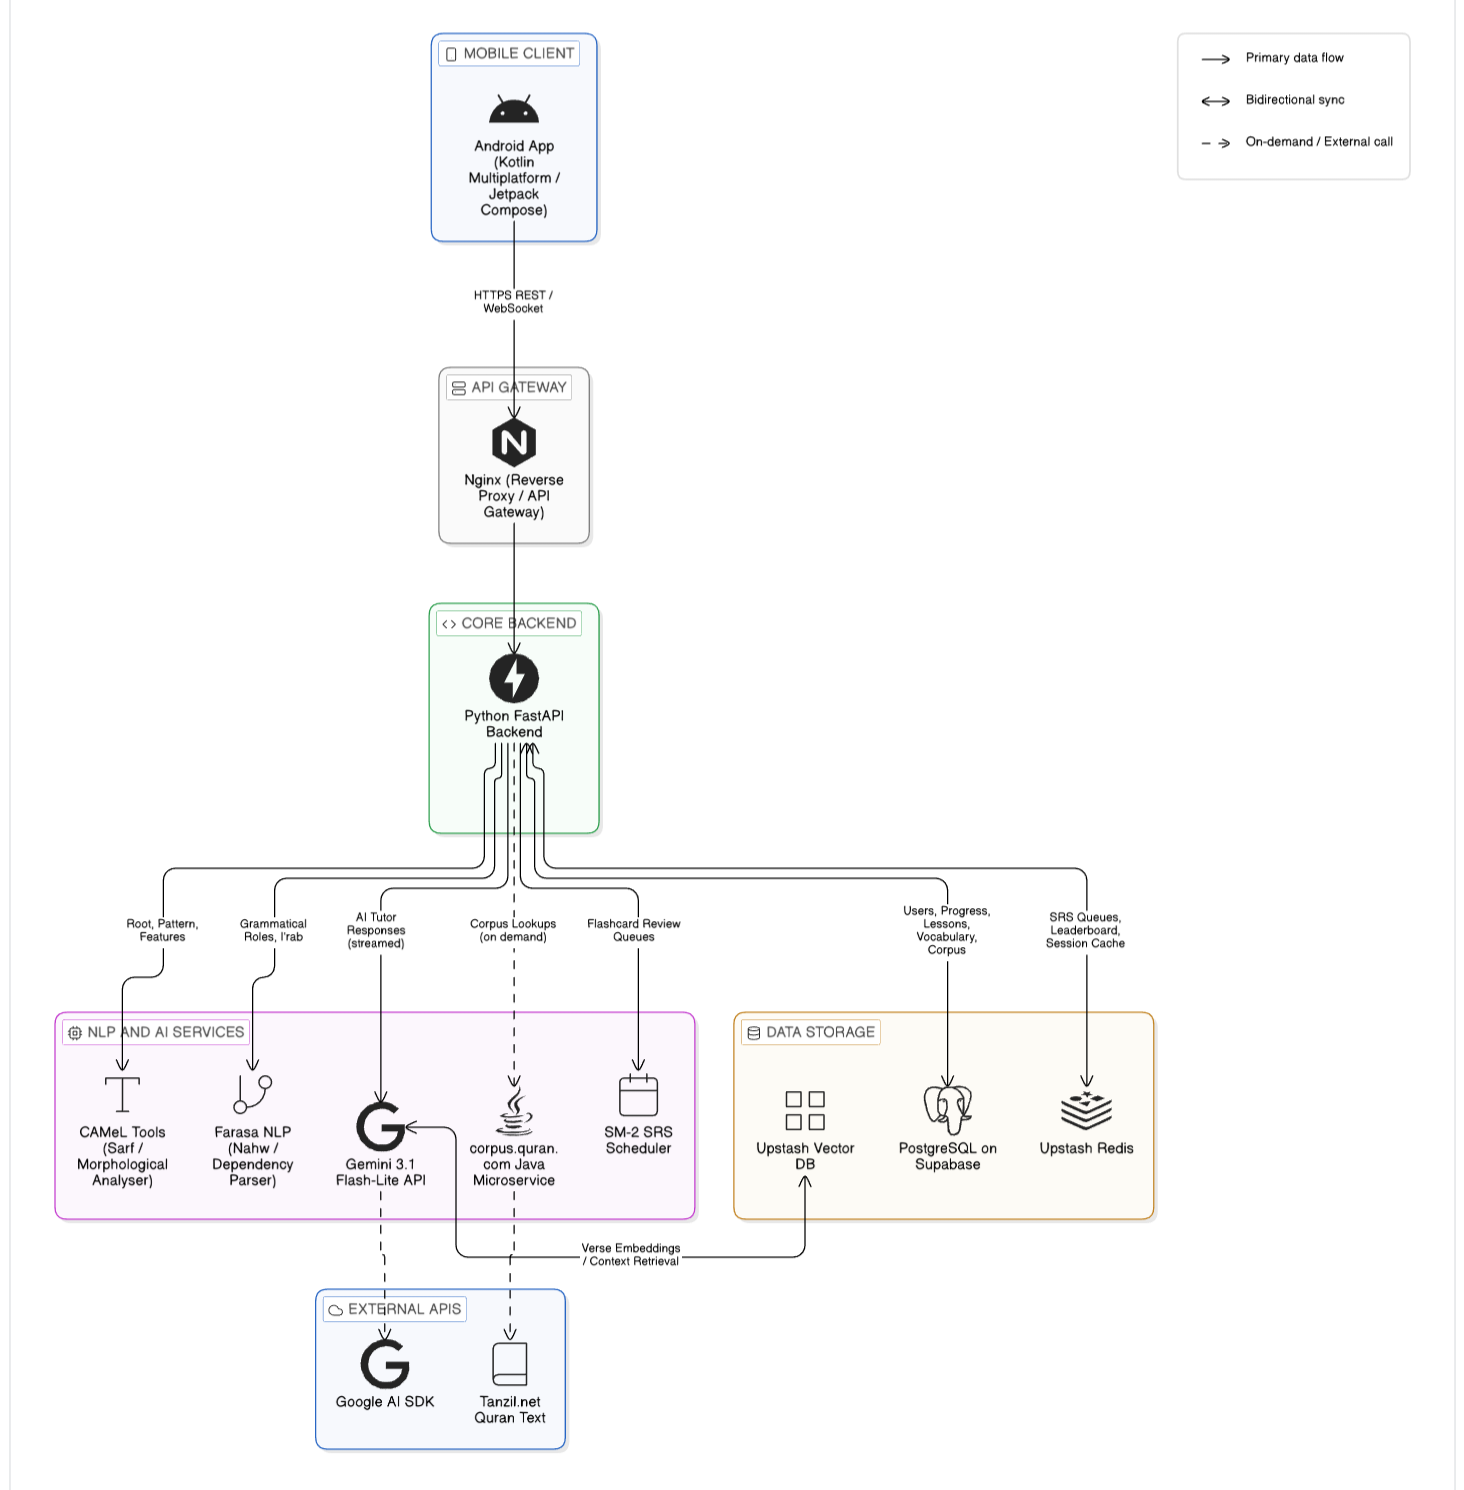
\includegraphics[width=0.85\linewidth]{system_architecture.png}
    \caption{End-to-End System Architecture of Jawhar Platform}
    \label{fig:arch}
\end{figure}

Jawhar bridges this divide by delivering a unified, AI-native platform designed specifically for self-paced comprehension of Quranic Arabic. As illustrated in Figure~\ref{fig:arch}, the platform provides immediate morphological decomposition, visual syntactic dependency mapping, an adaptive spaced repetition flashcard engine, and a conversational AI tutor capable of answering nuanced grammatical questions grounded in authoritative Quranic data.

\section{Literature Review}
Computational processing of Classical Arabic has evolved significantly over the past two decades. The Quranic Arabic Corpus (QAC) developed by Dukes and Buckwalter \cite{dukes2010dependency} established the foundational gold standard for Quranic morphological and syntactic annotation. However, the QAC covers approximately 40\% of deep dependency relations and presents data primarily in static web pages rather than modern interactive APIs. Recent developments such as the Extended Quranic Treebank (EQTB) \cite{eqtb2024} provide a complete, 43-column CoNLL-X annotation across all 132,736 Quranic tokens, formalizing 140 classical I'rab syntactic labels and elliptical constructions.

In morphological analysis, rule-based and statistical toolkits have achieved remarkable accuracy. CAMeL Tools \cite{obeid2020camel} provides a modular Python suite combining morphological modeling, disambiguation, and root extraction for both Classical Arabic and MSA. MADAMIRA \cite{pasha2014madamira} utilizes Support Vector Machines (SVMs) and n-gram language models to resolve clitic ambiguity and extract 13 distinct inflectional features. For clitic segmentation and high-speed processing, Farasa \cite{abdelali2016farasa} achieves state-of-the-art segmentation and dependency tagging, making it ideal for processing morphologically rich Quranic verses in real time.

For vocabulary acquisition, spaced repetition systems based on the forgetting curve have historically utilized SuperMemo's SM-2 algorithm \cite{wozniak1990sm2}. While effective, modern cognitive research demonstrates that the Free Spaced Repetition Scheduler (FSRS) \cite{ye2024fsrs} reduces review workloads by 20--30\% while achieving superior long-term retention stability.

In generative artificial intelligence, frontier large language models like Google's Gemini \cite{gemini2024} exhibit strong multilingual comprehension. Benchmarks such as IslamicMMLU demonstrate high accuracy in Quranic and Arabic reasoning; however, unconstrained generation risks hallucination. By integrating verified grounding data from Tanzil \cite{tanzil2024} and morphological engines via Retrieval-Augmented Generation (RAG), conversational tutors can maintain academic rigor.

\begin{table}[h!]
    \centering
    \small
    \caption{Comparative Analysis of Existing Systems vs. Jawhar}
    \label{tab:comparison}
    \begin{tabular}{|p{0.22\textwidth}|p{0.35\textwidth}|p{0.35\textwidth}|}
    \hline
    \textbf{Platform} & \textbf{Identified Weaknesses} & \textbf{Jawhar Proposed Solution} \\
    \hline
    \textbf{corpus.quran.com} & Desktop-only research UI; incomplete treebank; no interactive learning, practice, or AI tutor. & Modern cross-platform app (Android/iOS/Desktop/Web); full corpus integration with AI tutoring. \\
    \hline
    \textbf{Quranic App} & Rote vocabulary only; lacks grammatical breakdown, verb conjugation, and syntax parsing. & Deep Sarf root/pattern analysis and Nahw dependency annotation for every word. \\
    \hline
    \textbf{Kalaam} & Oversimplified grammar formulas; no conversational tutor; limited syntactic depth. & Classical Nahw role mapping (Mubtada, Khabar, Fa'il, Maf'ul) with interactive dependency trees. \\
    \hline
    \textbf{Tarteel AI} & Audio and recitation memorization only; zero grammar, vocabulary, or linguistic tools. & Comprehensive linguistic study platform focusing on textual comprehension and syntax. \\
    \hline
    \textbf{Duolingo / Babbel} & Modern Standard / Spoken Arabic only; unrelated vocabulary; no Classical/Quranic grammar. & Exclusively Classical Quranic Arabic curriculum grounded in verified Quranic text. \\
    \hline
    \textbf{Buruj / Kalimah} & Expensive teacher-led courses; synchronous scheduling; lack self-paced interactive software. & Free, autonomous, self-paced learning available 24/7 with instant AI feedback. \\
    \hline
    \end{tabular}
\end{table}

\section{Problem Statement}
Understanding Classical Arabic directly from the Quran presents four critical challenges for global learners:
\begin{enumerate}
    \item \textbf{Shallow Pedagogical Depth:} Existing digital applications focus almost exclusively on vocabulary flashcards, failing to teach the foundational grammatical disciplines of Sarf (word morphology) and Nahw (sentence syntax).
    \item \textbf{Accessibility \& Usability Gap:} Scholarly resources (such as corpus.quran.com) provide rigorous linguistic data but are locked in dense, desktop-only interfaces intended for academic linguists rather than independent students.
    \item \textbf{Prohibitive Cost \& Inflexible Scheduling:} Quality instruction in Classical Arabic is currently restricted to expensive, synchronous teacher-led institutes, leaving self-paced learners without structured guidance.
    \item \textbf{Linguistic Mismatch:} Mainstream language learning applications teach Modern Standard Arabic or regional dialects, which lack the syntactic complexity and classical vocabulary required to comprehend the Quran.
\end{enumerate}

\section{Project Objectives}
The primary objective of this project is to develop and evaluate \textbf{Jawhar}, an intelligent, cross-platform Classical Arabic learning system. Specific objectives include:
\begin{itemize}
    \item Develop an AI-driven \textbf{Sarf Engine} using CAMeL Tools that accepts any Arabic word and extracts its 3-letter root, morphological pattern (\textit{Wazn}), and full verb conjugation paradigm with $\ge 90\%$ benchmarked accuracy.
    \item Implement an interactive \textbf{Nahw Parser} using Farasa and classical I'rab mapping to annotate sentences with color-coded grammatical roles (\textit{Fa'il}, \textit{Maf'ul}, \textit{Mubtada}, \textit{Khabar}).
    \item Build a context-aware \textbf{AI Tutor} powered by Gemini Flash and grounded in verified Quranic corpora to provide accurate, pedagogical grammatical explanations without hallucinations.
    \item Implement a \textbf{Spaced Repetition System (SRS)} utilizing SM-2/FSRS algorithms to optimize Quranic vocabulary retention through daily adaptive review queues.
    \item Design an \textbf{Adaptive Learning Path} featuring an onboarding placement assessment and competency-based lesson progression aligned with classical curricula (e.g., Bayyinah Dream program).
    \item Deliver the platform as a unified \textbf{Kotlin Multiplatform} application (Android, iOS, Desktop JVM, Web) served by a high-throughput Python FastAPI backend.
\end{itemize}

\section{Proposed Solution}
Jawhar provides an integrated three-tier architecture:
\begin{itemize}
    \item \textbf{Cross-Platform Client:} A unified Compose Multiplatform UI codebase shared across Android, iOS, Desktop, and Web, offering authentic Arabic typography (Amiri Quran and Noto Naskh Arabic) with native RTL support.
    \item \textbf{Core REST Backend:} A FastAPI service orchestrating JWT authentication, user progress, spaced repetition schedules, and cached linguistic lookups via PostgreSQL and Redis.
    \item \textbf{NLP \& AI Microservices:} Python-based modules integrating CAMeL Tools and Farasa for real-time morphological analysis and syntax parsing, coupled with Google's Gemini Flash for streaming AI tutoring.
\end{itemize}

\section{Vision Statement}
To become the definitive open, accessible, and academically rigorous platform for learning Classical Arabic, enabling millions of learners worldwide to connect directly with the linguistic beauty and divine message of the Holy Quran.

\section{Scope}
\textbf{In-Scope:}
User authentication and profile management; full Quran browser with Uthmanic script and verified translations; Sarf root and pattern analyzer; Nahw grammatical role annotator; Gemini-powered conversational tutor; spaced repetition vocabulary system; adaptive curriculum unlock; automated evaluation against corpus.quran.com gold standards.

\textbf{Out-of-Scope (v1.0):}
Speech recitation analysis (Tajweed audio verification); live teacher video classrooms; secondary Qira'at variants; advanced rhetorical (\textit{Balaghah}) nuance classification.

\section{Methodology}
The development methodology follows an iterative, component-driven engineering approach organized into six distinct development milestones:
\begin{enumerate}
    \item \textbf{Foundation (M1):} Backend API scaffolding, PostgreSQL relational schema, Tanzil Quran corpus ingestion, JWT authentication, and KMP client project configuration.
    \item \textbf{SRS Engine (M2):} Memory retention scheduler, flashcard queue management, mastery tracking, and daily habit metrics.
    \item \textbf{Sarf Morphology Engine (M3):} CAMeL Tools pipeline integration, root extraction, pattern recognition, and conjugation generation.
    \item \textbf{Nahw Parser \& AI Tutor (M4):} Farasa dependency parser integration, color-coded role visualizer, and Gemini Flash tutoring pipeline with RAG safeguards.
    \item \textbf{Personalization \& Mobile (M5):} Assessment-based placement, curriculum prerequisites, and mobile client polish.
    \item \textbf{Evaluation \& Benchmarking (M6):} 30-participant empirical user study, linguistic accuracy benchmarking, and final deployment.
\end{enumerate}

\section{Tools and Technologies}
\begin{itemize}
    \item \textbf{Client Frontend:} Kotlin Multiplatform, Compose Multiplatform, Ktor Client 3.x, kotlinx.serialization, Amiri \& Noto Naskh Arabic fonts.
    \item \textbf{Backend Server:} Python 3.11, FastAPI, SQLAlchemy 2.0 (async), Alembic, Pydantic v2.
    \item \textbf{Databases \& Cache:} PostgreSQL 15+ (relational and corpus store), Redis 7+ (sessions, rate limits, SRS cache).
    \item \textbf{AI \& NLP Libraries:} CAMeL Tools, Farasa NLP, Google Gemini Flash API, Tanzil.net dataset, corpus.quran.com dataset.
    \item \textbf{DevOps \& Environment:} uv package manager, Docker, Nginx, GitHub Actions CI/CD.
\end{itemize}

\section{Applications of this Project}
\begin{itemize}
    \item \textbf{Self-Paced Quranic Learners:} Independent students seeking structured, accessible comprehension of the Quran without full-time enrollment in traditional seminaries.
    \item \textbf{Islamic Educational Institutions:} Supplementary classroom tool for madaris and Islamic schools to provide students with automated grammar drills and vocabulary homework.
    \item \textbf{Academic Researchers:} Standardized REST API interface for exploring Quranic morphology, roots, and syntax in computational linguistics research.
    \item \textbf{Converts to Islam and Non-Arabic Speakers:} Gentle, beginner-friendly ramp into Classical Arabic syntax without intimidation.
\end{itemize}

\section{WBS and Gantt Chart}
The project follows a structured 9-phase execution plan spanning requirements, NLP pipelines, core backend, mobile and cross-platform clients, integration testing, empirical evaluation, and documentation. The project timeline is visualized in Figure~\ref{fig:gantt}.

\begin{figure}[h!]
    \centering
    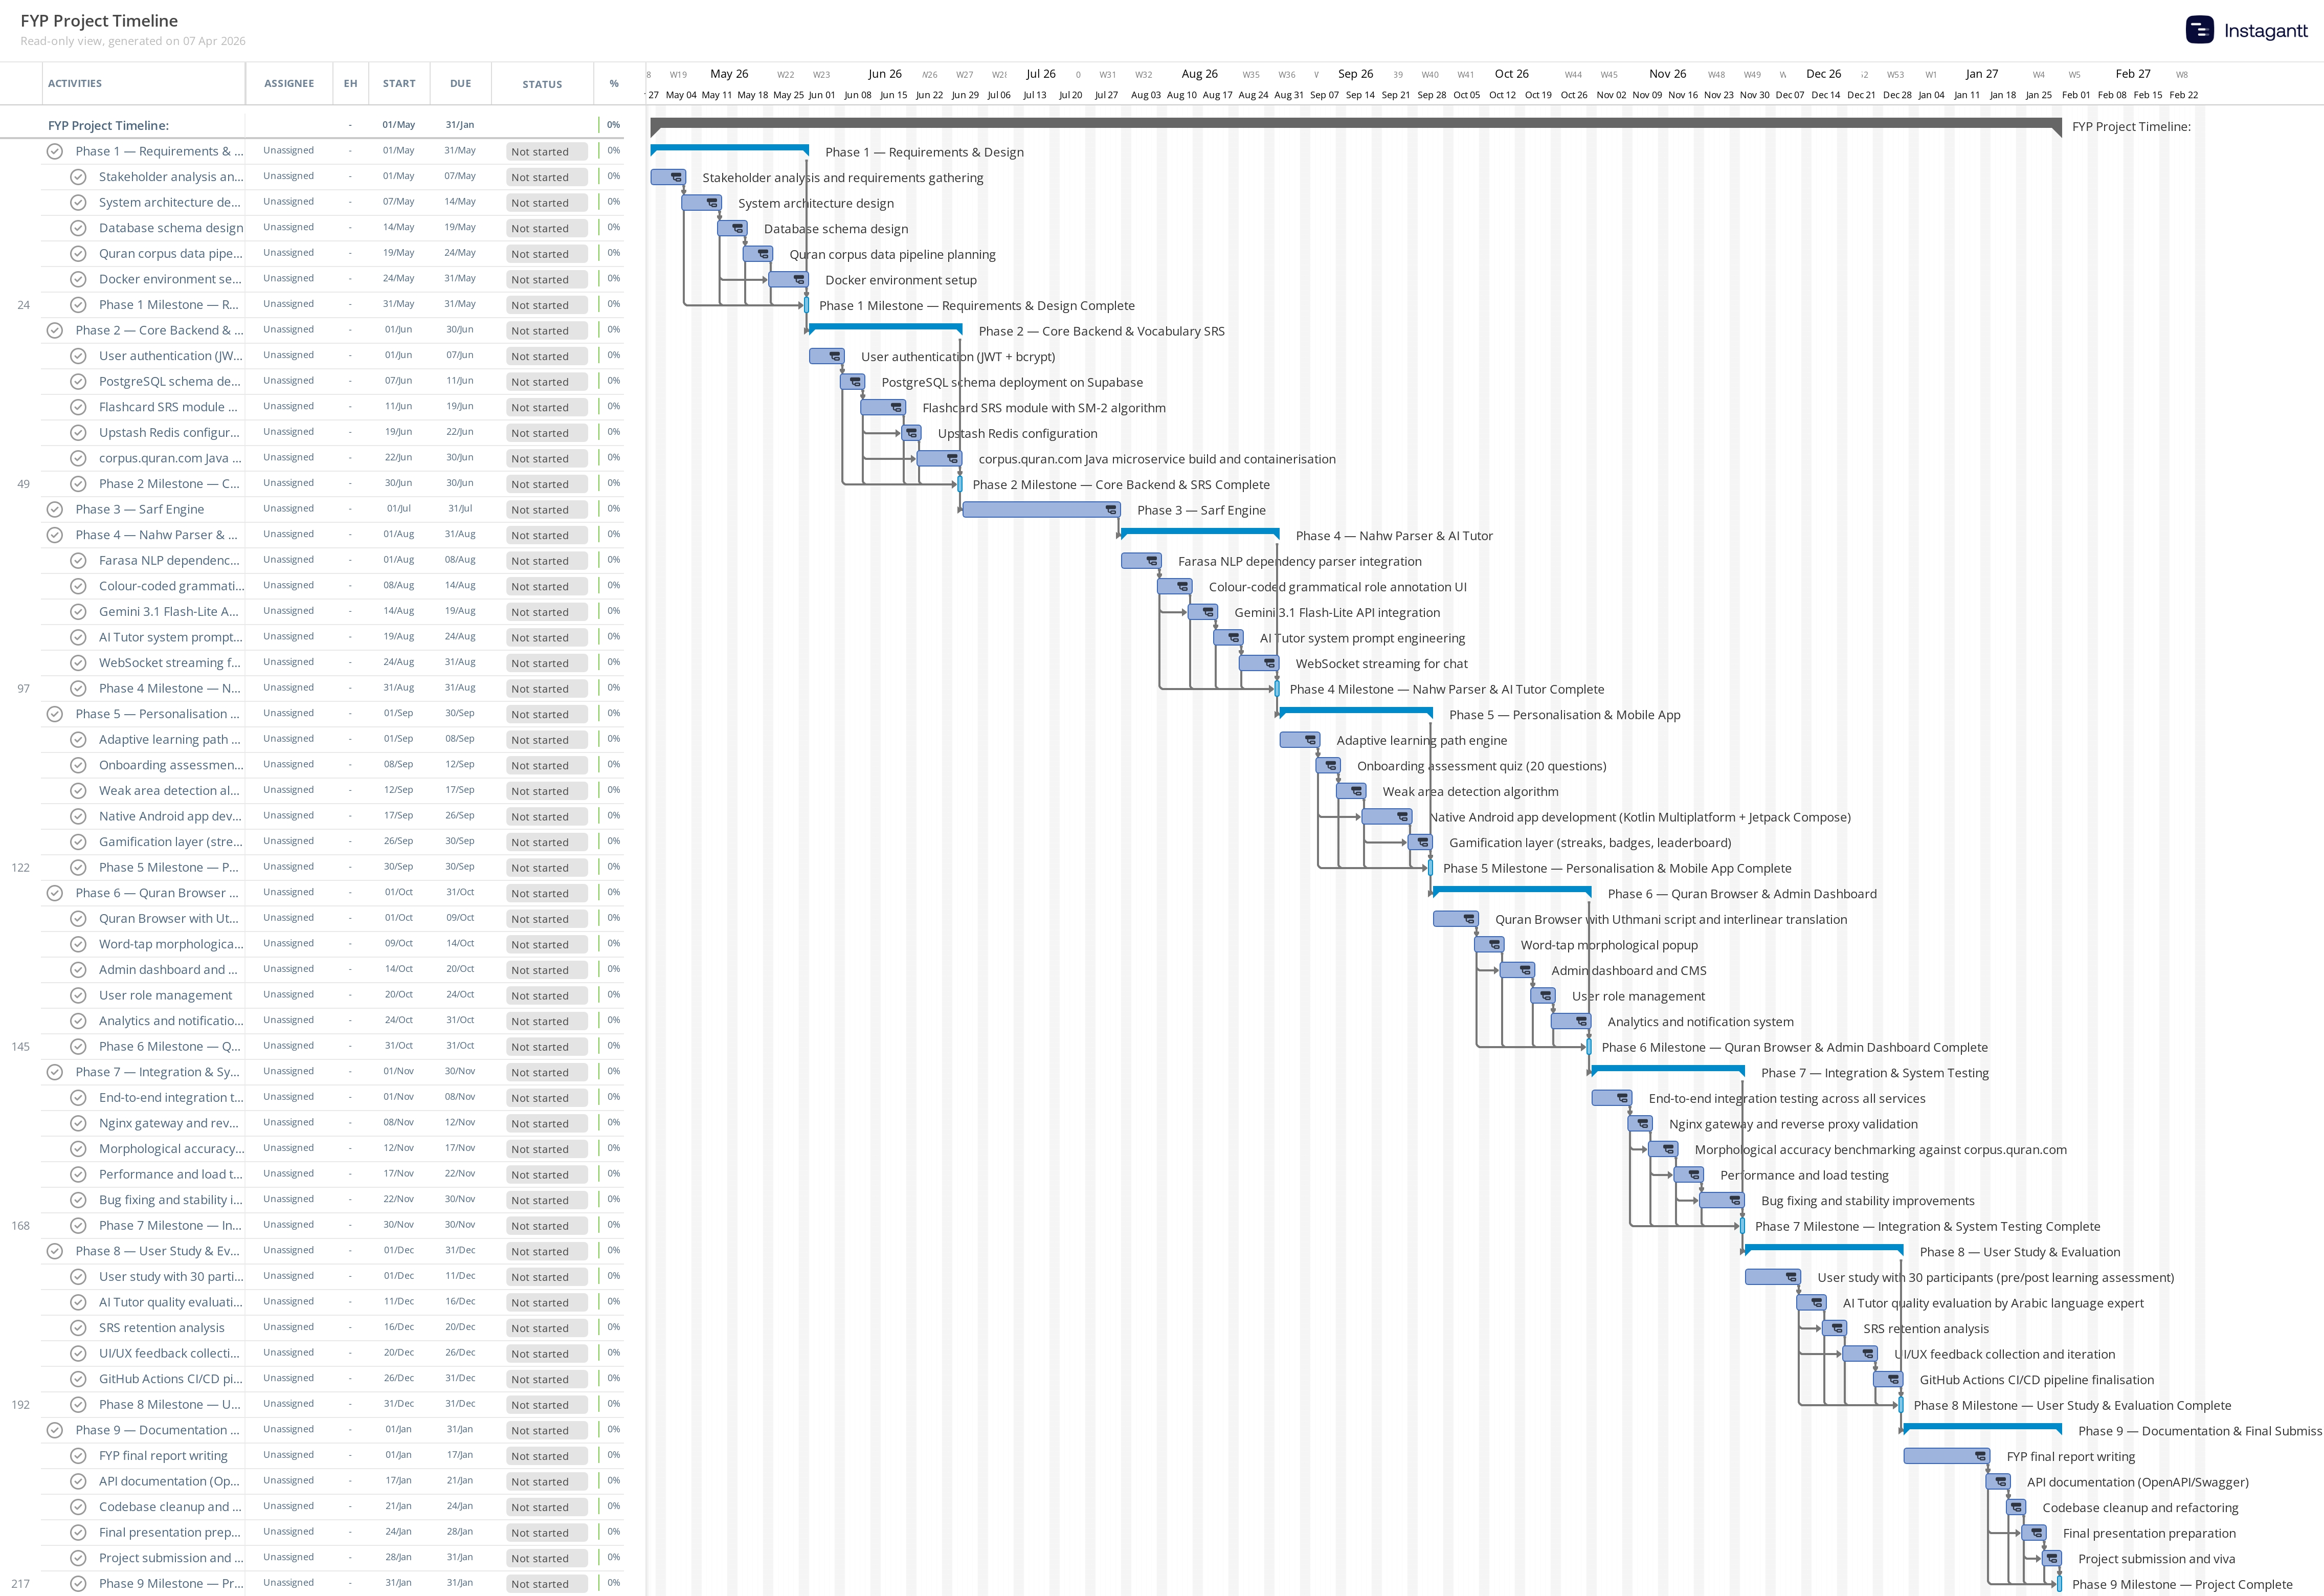
\includegraphics[width=0.98\linewidth]{gantt_chart.png}
    \caption{Work Breakdown Structure and Detailed Gantt Chart Timeline}
    \label{fig:gantt}
\end{figure}

\section{Mockups}
The user interface adheres to a calm, scholarly Islamic aesthetic utilizing deep emerald green (\texttt{\#0B6B4F}) and warm sand (\texttt{\#F7F4EE}) tones with authentic Quranic typography. The mobile interface provides seamless word-by-word morphological tap sheets, color-coded syntactic legends, flashcard review decks, and streaming AI tutor chats.

\newpage
\bibliography{final}
\newpage
\end{document}
